\documentclass[10pt]{report}
\usepackage{hyperref}
\usepackage[english]{babel}
\usepackage{graphicx}


\renewcommand\thesection{\arabic{section}}
\renewcommand\thesubsection{\thesection.\arabic{subsection}}

\newcommand*{\titleGM}{\begingroup % Create the command for including the title page in the document
\hbox{ % Horizontal box
%\hspace*{0.01\textwidth} % Whitespace to the left of the title page
\rule{1pt}{\textheight} % Vertical line
\hspace*{0.05\textwidth} % Whitespace between the vertical line and title page text
\parbox[b]{0.75\textwidth}{ % Paragraph box which restricts text to less than the width of the page

{\noindent\Huge\bfseries User Interface \\Design}\\[2\baselineskip] % Title
{\large \textit{Final submission}}\\[4\baselineskip] % Tagline or further description
{\Large \textsc{Arno De Witte}}\\
{\Large \textsc{Kwinten Pardon}}

\vspace{0.5\textheight} % Whitespace between the title block and the publisher
}}
\thispagestyle{empty}
\endgroup}

\begin{document}

\titleGM
\clearpage\setcounter{page}{1}

\section{Application Description}
Our application eliminates the search for contact information for the professor in charge of a certain course. It enables the student to ask a question, related to a course he follows, in a fast and straightforward manner. The application will also list the questions asked by his fellow students and the given answers. This way, a knowledge base
per course is formed.

\section{Users}
The application is based on 2 existing user classes. It contains students who are taking courses on the one hand and professors in charge of said courses on the other. The application does not require a super user since the application is based in a university environment and all data should be imported from other already existing databases or applications.

\subsection{User Classes}

\subsubsection{Student}

\begin{tabular}{ | l | p{10cm} |}
\hline
\textbf{Type} & Primary User \\ \hline
\textbf{Usage frequenty} & Daily Use \\ \hline
\textbf{Computer experience} & Novice \\ \hline
\textbf{Application familiarity} & From novice as first degree bachelor student to competent performer in second degree master student. Application shows familiarities with other applications such as Pointcarre\\ \hline
\textbf{Usage} & discretionary\\ \hline
\textbf{Number of users} & 12.000+\\ \hline
\textbf{Motivation} & 
	\begin{itemize}
		\item Positive 
		\begin{itemize}
			\item eliminates the search for contact information
		\end{itemize}
	\end{itemize} \\ \hline
\textbf{tasks} & 
	\begin{itemize}
		\item Watch overview of courses (number of new questions / new answers per course)
		\item Watch overview of questions statust per course (answered, follow-up question unanswered, unanswered)
		\item Ask a question regarding a course (public or private)
		\item Mark a question as answered (only if he is the original person who asked the question)
		\item Ask follow-up question
	\end{itemize} \\ \hline
\end{tabular}

\subsubsection{Professor}

\begin{tabular}{ | l | p{10cm} |}
\hline
\textbf{Type} & Primary User \\ \hline
\textbf{Usage frequenty} & Daily Use \\ \hline
\textbf{Computer experience} & Novice \\ \hline
\textbf{Application familiarity} & Competent Performer due to similarities with other systems such as Pointcarre \\ \hline
\textbf{Usage} & Mandatory\\ \hline
\textbf{Number of users} & 700\\ \hline
\textbf{Motivation} & 
	\begin{itemize}
		\item Positive 
		\begin{itemize}
			\item Questions, separated by class instead of cluttered in email inbox
			\item Preventing duplicate questions by making a question public
		\end{itemize}
		\item Negative 
		\begin{itemize}
			\item Might prefer email
		\end{itemize}
	\end{itemize} \\ \hline
\textbf{tasks} & 
	\begin{itemize}
		\item Watch overview of courses (number off new questions, follow up questions per course)
		\item Watch questions per course (unanswered new, unanswered follow up question, answered)
		\item Filter questions (unanswered new, unanswered follow up question, answered)
		\item Change private question to public
		\item Answer (follow-up) question
		\item discard question (refuse to answer)
	\end{itemize} \\ \hline
\end{tabular}

\subsection{User Models}

\begin{center}
	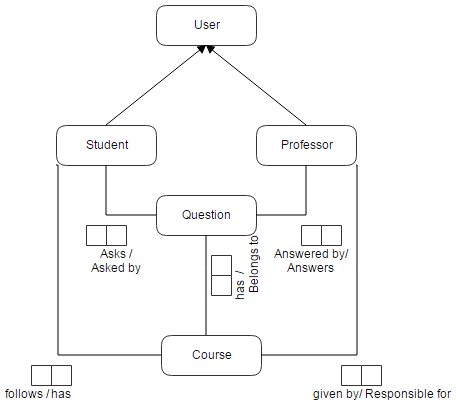
\includegraphics[scale=1]{img/orm.png}
\end{center}

\subsection{Usability Requirements}
\begin{itemize}
	\item Users should be able to log in, within 10 seconds using their university credentials.
	\item Users should be able to navigate to the right course within 30 seconds.
	\item Students should be able to start the process of asking a question within 10 seconds. (Time on completing this task is dependant on the complexity of the question).
	\item Professors should be able to start the process of answering a question within 10 seconds. (Time on completing this task is dependant on the complexity of the question).
	\item Users should be able to find a question within 10 seconds. (only if they're already in the right course. If not time required to navigate to the right course should be included making it 40 seconds)
	\item Users should be able to change the status of a question instantly, provided the question already has been found.
	\item Users should be able to change the visibility of a question instantly, provided the question already has been found.
	\item Users should be able to log out within 5 seconds.
\end{itemize}

\section{CTT}

\section{Style Guide}
For our style guide we based ourselves upon the material design guidelines created by Google\footnote{\url{https://www.google.com/design/spec/material-design/introduction.html}}. These are design guidelines specifically made for use on all sorts of different screen sizes. It uses a flat simple design that aims to be intuitive. Implementation for these guidelines can be found in numerous of Google products and in a lot of other applications, both mobile and on the web.\\
These guidlines are also implemented in some web frameworks, we used material design lite which is implemented by google. We based this prototype upon one of the templates provided by default from this framework.\\

Below are some of the interaction as defined by our style guide:\\
\begin{itemize}

\item Standards for window interaction: Handled by the browser.
\item Standard window layout: A top bar with the title of the current page (equal to the current course in our application). This top bar should contain the main actions possible on the current page. In our prototype these are search and a action drop down menu. A menu bar containing the main pages (the different courses), information of the current user on top and if applicable a help button. This menu bar should be collapsed on devices with a small screen width.
\item Standards for buttons and menus: Buttons should have bright colour and if applicable an icon to indicate their action. If a default icon (material design provides a set of icons\footnote{\url{https://design.google.com/icons/}}) can not be found for the action, the button may contain text. For actions that add main content objects such as seen in the current screen, a so called FAB (floating action button) button should be provided in the bottom right of the screen. For toggles, icons or sliders can be used. When creating an item or for use in a form, sliders are used. When listing the action in an overview a icon should be used.\\
Menu's should be indicated with the 3 dot icon. They should drop down, have a white background and have their items as text. When all items of a menu can be illustrated with an icon, icons may be used. However this is not the case in the prototype.\\
Whenever using an icon, the usage of a tool tip (a small grey box with some helpful text that pops up when hovering over the icon) is highly recommended but not required. 
\item Standards for use of keyboard: When in a form, the tab key is used to go to the next item in the form. The enter key indicates that the user wants to commit his or hers input. These are standards widely used on the web.
\item Standards for text: In material design the roboto font is used\footnote{\url{https://www.google.com/fonts/specimen/Roboto}}. This font is used because it performs well on different screen sizes. The default size is 14 pixels for text. For titles the font size may very depending on which kind of title. The colour of the text depends on its background. For darker background (such as the sidebar) white or light grey text is used. When indicating additional information about a content object (for example the author of a question) it's recommended to use an italic font style to indicate that the text is a piece of meta information.
\item Standards for colour: Colour can be used to indicate the difference between areas. For example the difference in colour between the title of a question and the description or the difference between the main panel and the sidemenu. Items that should draw attention, such as the FAB, should have a bright colour.
\item Standards for user objects: The only relevant user object for this prototype is a question. Questions are listed in a list, each question should be initially collapsed to indicate it is not in use. When in the collapsed state, only the question title is visible. Users can however perform actions (toggle visibility, open/close) on them. When opening a question the description and potential responses become visible. Also if the question is open, the user gets the response form.
\item Standards for integration of information from other applications: Users can use the copy paste feature in their browser to copy text into the input fields.  
\end{itemize}


\section{Design Report}

\section{Evaluation Report}
When designing this prototype we started out by sketching the design on paper. We tried to make the best possible model to fit our requirements. Then we created the wireframes. These are quite hard to iteratively improve, therefore we set out to create a working prototype as fast as possible. When we created the prototype we each evaluated the parts of the prototype each member had created. In this phase already some improvements were made. For example the email verification was improved by adding the support to just press enter.\\
In a second phase the prototype was send to another group for evaluation. There evaluation was very helpful as it provided an independent view on our prototype. The group pointed out some flaws in our prototype, such as the meaning of each icon and the fact that the placement of some buttons might be odd for new users. Therefor we added some tool tips and a help button which reveals an overlay that points to all features that might not be obvious to new users. Other small improvements were made based on this report which is included with this report.


\end{document}